\documentclass[a4paper,12pt]{report}
\setcounter{secnumdepth}{5}
\setcounter{tocdepth}{3}
\newcounter{ZhRenew}
\setcounter{ZhRenew}{1}
\newcounter{SectionLanguage}
\setcounter{SectionLanguage}{1}
\input{/usr/share/latex-toolkit/template.tex}
\begin{document}
\title{海洋學}
\author{沈威宇}
\date{\temtoday}
\titletocdoc
\ch{海洋學(Oceanography)}
\sct{海洋的結構}
\ssc{壓力}
每下降10公尺海水壓力約增高1 bar。
\ssc{鹽度(Salinity)}
\sssc{鹽度}
每公斤水體中溶解鹽類公克數。海水(seawater or sea water)的平均鹽度約35\textperthousand。
\sssc{實用鹽度(Practical Salinity Scale, PSS}
基於溫鹽探儀(Conductivity Temperature Depth, CTD)測得的電導率比值(Conductivity Ratio),即海水電導率與標準鉀氯溶液電導率的比值的鹽度測量,並有多個修正項以使接近傳統鹽度,無單位或實用鹽度單位(Practical Salinity Unit, psu)。
\sssc{氯度(Chlorinity, Cl)}
令海水樣本中所有鹵素沈澱的所需銀的質量。由於海水中主要離子比例固定,可從氯度推算鹽度。
\sssc{經驗公式}
\[S \approx 0.03 + 1.805\text{Cl}\]
其中$S$為鹽度,Cl 為氯度。
\sssc{海水的成分}
鹽度 35 的海水其成分約為:
\begin{longtable}[c]{|c|c|}
\hline
成分 & 濃度 (mol/kg) \\\hline\endhead
\ce{H2O} & 53.6 \\\hline
\ce{Cl-} & 0.546 \\\hline
\ce{Na+} & 0.469 \\\hline
\ce{Mg^{2+}} & 0.0528 \\\hline
\ce{SO4^{2-}} & 0.0282 \\\hline
\ce{Ca^{2+}} & 0.0103 \\\hline
\ce{K+} & 0.0102 \\\hline
\ce{C}$_\tx{T}$ & 0.00206 \\\hline
\ce{Br-} & 0.000844 \\\hline
\ce{B}$_\tx{T}$ & 0.000416 \\\hline
\ce{Sr^{2+}} & 0.000091 \\\hline
\ce{F-} & 0.000068 \\\hline
\end{longtable}\FB
其中 \ce{C}$_\tx{T}$ 為總無機碳(total inorganic carbon, TIC),主要為碳酸根\ce{CO3^{2-}}、碳酸氫根\ce{HCO3-}、碳酸\ce{H2CO3}與二氧化碳\ce{CO2};\ce{B}$_\tx{T}$ 為總硼(total boron),主要為硼酸根\ce{BO3^{3-}}、硼酸氫根\ce{HBO3^{2-}}、硼酸二氫根\ce{H2BO3-}、硼酸\ce{H3BO3}與四硼酸\ce{B4O5(OH)4^{2-}}。
\subsubsection{鹽類移出入水圈之平衡}
\begin{itemize}
\item 陰離子來源:主要為火山活動,亦有大氣沉降等。
\item 陽離子來源:主要為岩石風化作用。
\item 鹽類移出:被海洋生物利用轉為殼骨,或因生物或化學作用沉澱,後可能因板塊作用抬升出海平面、隱入地函或形成變質岩等。
\item 目前海洋鹽類移出與移入約達平衡。
\end{itemize}
\subsubsection{海表鹽度的影響因素}
\begin{itemize}
\item 與鹽度正相關的因素:如海水蒸發、結冰。
\item 與鹽度負相關的因素:如降水、淡水久留注入、融冰。
\item 鹽類移出入水圈之量在現今相較於前二項在短時間大空間尺度下影響甚小。
\end{itemize}
\sssc{海表鹽度分布}
\begin{figure}[H]
    \centering
    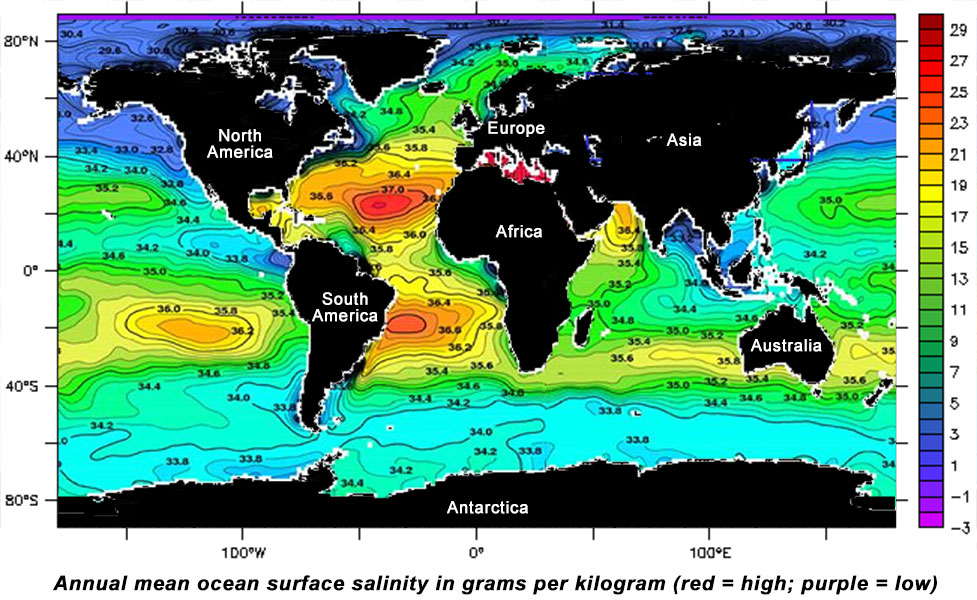
\includegraphics[width=0.9\textwidth]{SSS.jpg}
    \caption{Sea-surface salinity (SSS)}
\end{figure}\FB
全球海表鹽度大多約32\textperthousand  至38\textperthousand 。
\begin{itemize}
\item 副熱帶海域因蒸發大於降水故表層鹽度最高。
\item 赤道地區因蒸發小於降水故表層鹽度較副熱帶小。
\item 高緯度海域因蒸發小於降水與海冰熔化使表層鹽度最低。
\item 靠近陸地的邊緣海受周遭環境影響,等鹽線常較密,淡水注入會使表層鹽度下降。如南海與東海因降水強烈與淡水注入,表層鹽度僅約32\textperthousand ;地中海與紅海因蒸發旺盛與半封閉海域,表層鹽度高達38\textperthousand 以上。
\item 大西洋蒸發量減去降水量較太平洋大,故大西洋鹽度較太平洋高。
\item 洋流也會影響鹽度。如北大西洋暖流讓歐洲西岸等鹽線向高緯度延伸,使歐俄平原北岸仍可有34\textperthousand 以上的鹽度。
\item 地中海蒸發量大於大西洋,鹽度較高,在直布羅陀海峽形成雙層對流,表層海流由西向東,底層海流由東向西,前者密度較後者小,總水流量為西向東,總鹽流量為由東向西。
\end{itemize}
\ssc{密度}
海水垂直分布由密度決定,而密度受到溫度、鹽度與壓力影響,其中溫度與密度負相關,鹽度與密度正相關,壓力與密度正相關。
\sssc{經驗公式}
密度$\rho$、溫度$T$、鹽度$S$、壓力$P$、零壓力密度$\rho_{SW}$、經驗常數係數$K_1$、$K_2$、$K_3$、$K_4$、$K_5$、$a$、$b$、$c$、$d$、$e$:
\[\rho(T,S,P) = \rho_{SW} + \frac{P(K_1 + K_2P + K_3P^2)}{1 + K_4P + K_5P^2}\]
\[\rho_{SW} = \rho_0 + aS - bT + cT^2 - dT^3 + eS^2\]
\sssc{海表密度分布}
\begin{figure}[H]
    \centering
    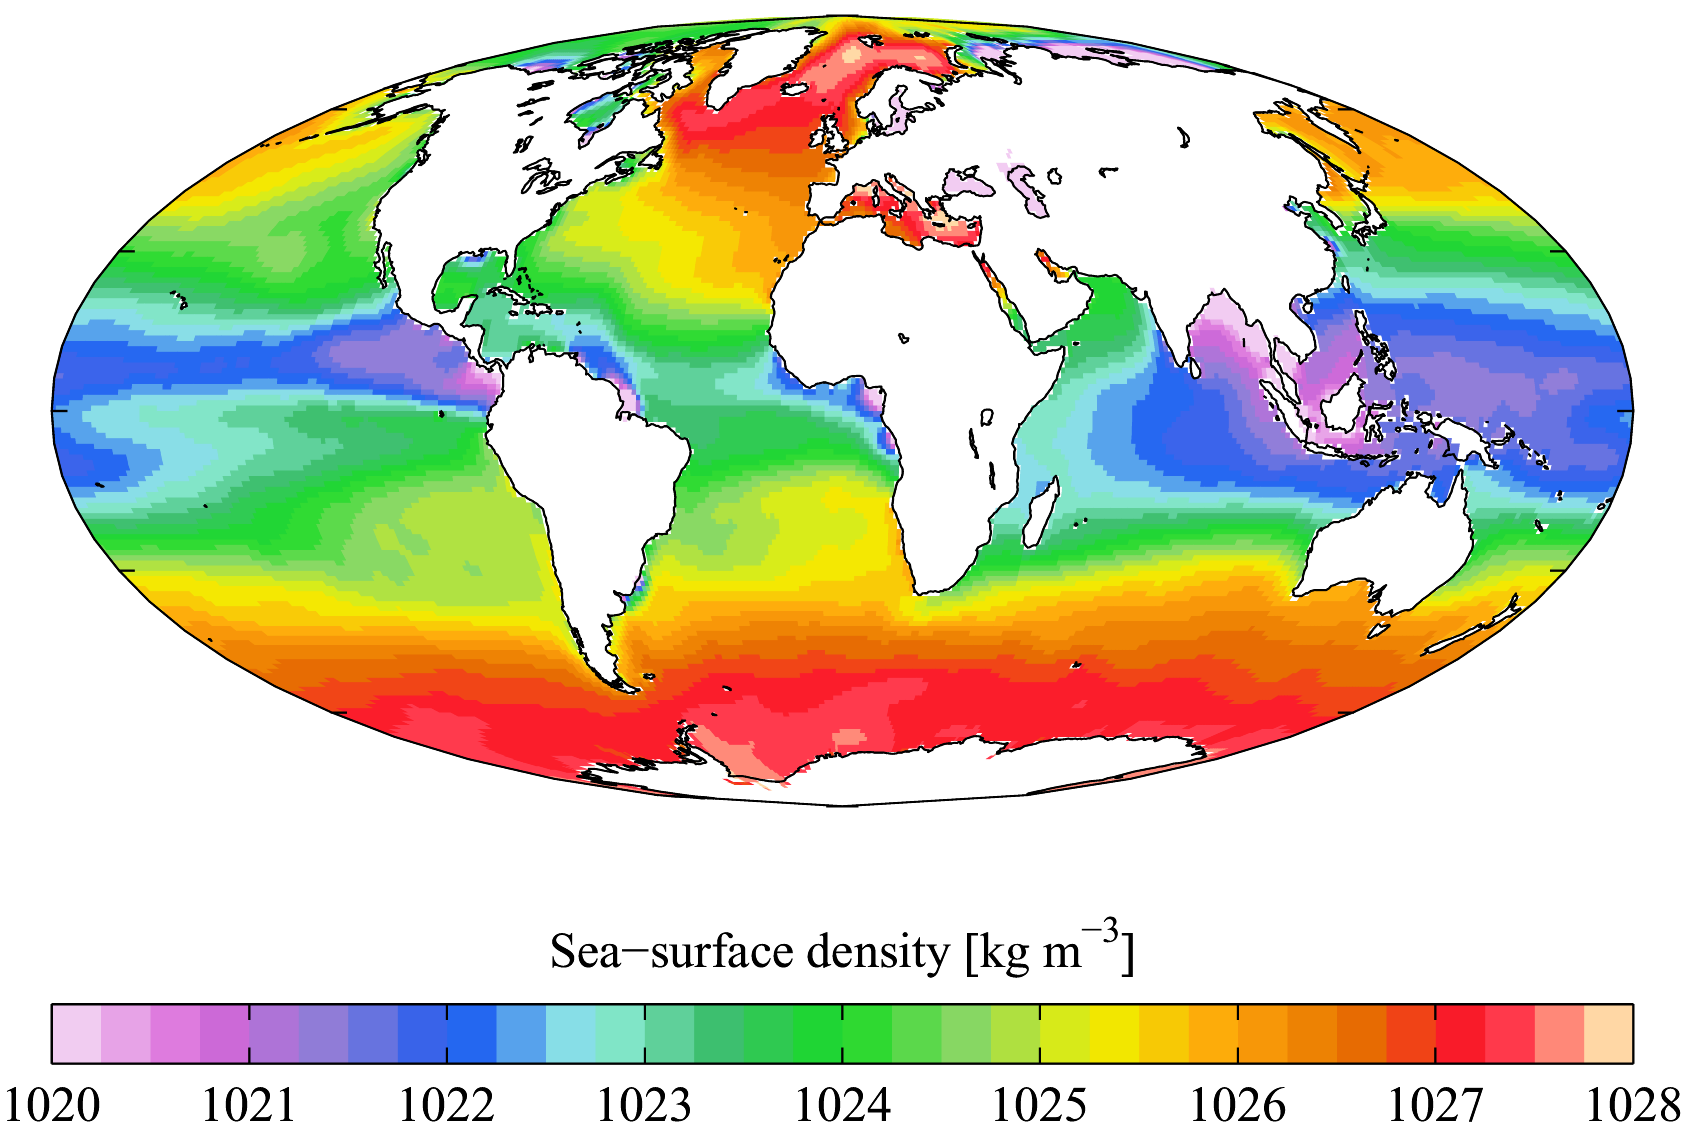
\includegraphics[width=0.9\textwidth]{SSD.png}
    \caption{Sea-surface density (SSD), Plumbago}
\end{figure}\FB
\ssc{溫度}
\sssc{海表溫度的影響因素}
海洋表面的熱量主要來自太陽輻射,故海表溫度與緯度負相關,等溫線略平行於緯度線,但亦受海流與湧升流影響,並有季節變化,夏季海溫較高。
\sssc{海表溫度分布}
\begin{figure}[H]
    \centering
    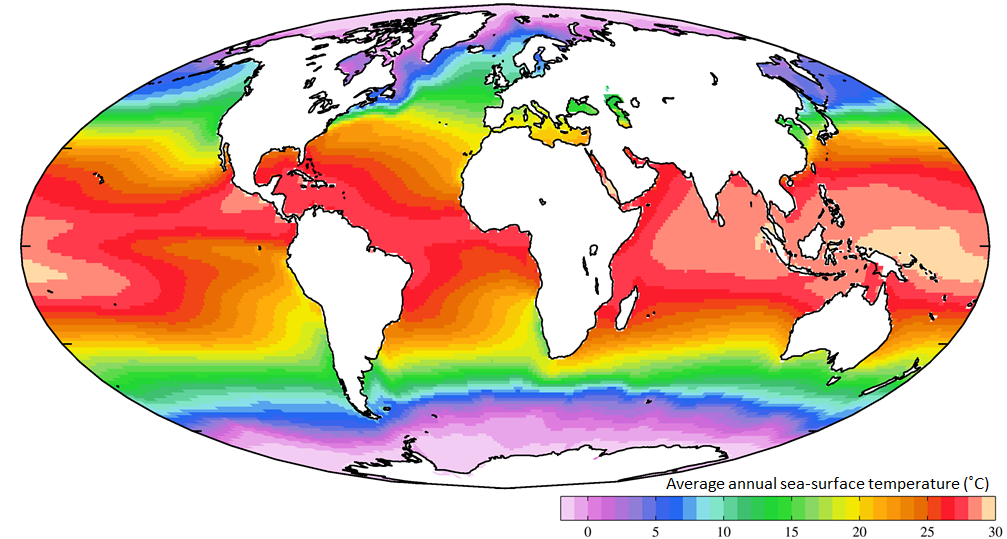
\includegraphics[width=0.9\textwidth]{SST.png}
    \caption{Sea-surface temperature (SST), Plumbago}
\end{figure}\FB
\begin{itemize}
\item 赤道可達28°C,兩極可達0°C以下。
\item 黑潮和墨西哥灣暖流讓北太平洋和北大西洋低緯西側的等溫線向高緯度延伸。
\item 北大西洋暖流讓歐洲西岸等溫線向高緯度延伸。
\item 加利福尼亞涼流、秘魯涼流、加那利涼流、本吉拉涼流讓北太平洋、南太平洋、北大西洋和南大西洋東側的等溫線向低緯度延伸。
\item 秘魯湧升流降低該處海溫。
\item 信風與北太平洋、南太平洋暖流將暖水推往西側堆積形成西太平洋暖水區。
\end{itemize}
\ssc{溫鹽圖(Temperature-salinity diagrams, T-S diagrams)}
縱軸表溫度,橫軸表鹽度,其上的眾多弧線(如有)表等密度線。其上記錄的數據為不同深度、位置或水團的溫度和鹽度,記錄同一位置不同深度者常繪製為溫鹽曲線,上標以深度。
\bct\bfH\ctr\icg[width=0.9\tw]{T-Smass.png}\caption{Christina Cardona, 2023. \href{https://opencontent.ccbcmd.edu/ccardona2023oceanography/chapter/7-7-thermohaline-circulation}{https://opencontent.ccbcmd.edu/ccardona2023oceanography/chapter/7-7-thermohaline-circulation}}\ef\FB\ect
\bct\bfH\ctr\icg[width=0.9\tw]{T-S1.png}\caption{Wrfrancis, 2017.}\ef\FB\ect
\sssc{混合增密作用}
兩水團混合,若溫度與鹽度為線性平均,則密度小於其密度之線性平均。
\ssc{水團(Water mass)}
指在水域中,一群具有相似溫度、鹽度、密度等物理特性的水體,與周圍的水體有所區別。水團通常由特定的形成區域(formation region)產生,然後沿著洋流擴散到其他地區。
\ssc{海水分層}
\sssc{混合層(Mixed layer)/表層(Surface zone)}
\begin{itemize}
\item 深度通常在0至50到200米之間。
\item 由於風和波浪的作用,這一層的水體混合較為均勻。
\item 溫度和鹽度相對穩定,並且受到季節變化的影響較大。
\end{itemize}
\sssc{溫躍層/斜溫層(Thermocline)}
\begin{itemize}
\item 深度通常在混合層底至800到1000米之間。
\item 低緯度溫度隨深度迅速下降,高緯度溫度隨深度下降不明顯,中緯度隨季節變動。
\item 在溫度隨深度下降明顯處,使得上下水體之間的交換變得困難,形成一個明顯的屏障,但在高緯度上下分層不明顯,可形成對流。
\end{itemize}
\sssc{密度躍層(Pynocline)}
\begin{itemize}
\item 深度大致與溫躍層相同。
\item 密度隨深度迅速上升。
\end{itemize}
\sssc{鹽躍層(Halocline)}
\begin{itemize}
\item 深度大致與溫躍層相同。
\item 高緯度區域鹽度隨深度迅速上升,低緯度區域鹽度隨深度迅速下降,中緯度不明顯。
\end{itemize}
\sssc{深水層(Deep zone)}
\begin{itemize}
\item 深度在溫躍層底至海底。
\item 溫度、鹽度、密度隨深度變化較小,水體相對穩定。
\item 密度較高,約1.03g/cm$^3$。
\item 除火山活動地區外,約1至2攝氏度。海水因為鹽類與壓力,密度最大的溫度低於4攝氏度。
\item 鹽度約35\textperthousand。
\end{itemize}
\sct{海水的運動}
\ssc{分類}
\begin{itemize}
\item 週期:洋流週期數月至數年。潮汐週期數小時。波浪週期數十秒。
\item 傳遞物質或能量:洋流傳遞物質與能量。波浪和潮汐主要傳遞能量。潮汐常被認為是一種特殊的波浪現象,但潮汐的動力學與一般波浪有所不同,因為潮汐主要由天體引力驅動。
\item 洋流(Ocean current)/海流:指海洋中具有較大規模、流向穩定的海水流動。
\item 波浪(Wave):指海面上起伏的現象,能夠傳遞能量,但不會伴隨大量的物質傳遞。
\item 潮汐(Tide):指由月球和太陽引力造成的海水週期性升降運動。
\end{itemize}
\ssc{波浪}
\begin{itemize}
\item 波浪:水面起伏的現象,水分子作圓周運動並傳遞能量,而不傳遞介質。
\item 風浪:風造成的波浪。受風區(風域)愈大或受風時間愈長,風浪波長、週期、能量、浪高與可傳遞距離愈大。
\item 湧浪/長浪:大洋受風區形成波長與波速不一的風浪,其中波長達數十公尺以上的長浪稱湧浪,能量衰減慢且波速快,離開受風區後仍可繼續傳遞。
\item 波浪擴展(Wave shoaling):當水深變淺,波浪會受到海底摩擦力影響而減速,出現後浪追前浪的現象,波長逐漸縮短,波高逐漸增加。令$h$為水深,$g$為重力加速度量值,$k$為波數,根據 Airy wave theory ,理想水面波相速度為$\sqrt{\frac{g}{k}\tanh\qty(kh)}$,$h>\frac{1}{2}\lambda$的深水波常近似為$\sqrt{g}{k}$,$h<\frac{1}{20}\lambda$的淺水波常近似為$\sqrt{gh}$。
\item 碎波/碎浪:一旦波高高於波長約七分之一,就會因為接近海底處受到海底摩擦力前進速度較慢、正位移處不受摩擦力前進速度較快,而崩塌形成碎波,能量轉化為泡沫、聲音、熱、沿岸流與離岸流等。沿海處水淺,波高高,故形成碎波帶,是改變海岸地形的主要侵蝕外營力。波浪能量強大的海岸以侵蝕作用為主,海岸線較為崎嶇,多岩岸;波浪能量微弱的海岸以堆積作用為主,海岸線較為平直,多沙岸。
\item 海嘯(Tsunami):由水下地震、火山爆發、海底滑坡或其他地質事件等非氣象因素引起的海洋波浪。具有非常長的波長(通常超過100公里)和極大的能量,在深海中速度可以達到500-800公里每小時,$h<<\frac{1}{2}\lambda$,由於波長很長波高通常不大(通常低於1米),在海面上不易察覺。當海嘯波浪進入淺水區域時,波速減慢,波高增大。在沿海地區,海嘯波高可能會劇增,形成數米到數十米的水牆。若波谷先到達岸邊,會造成海水後退,應盡快逃離至高處;若波峰先到達岸邊則沒有逃離時間。
\item 折射:由於近岸的波浪受到海底地形影響波速,波浪前進方向折射向水深較淺處。
\item 岬灣:因波浪折射,能量往岬角匯聚集中,使其侵蝕力趨向使海岸平直。
\item 沿岸流(Longshore current):前進方向平行於海岸的波浪,通常因波浪折射形成。
\item 突堤效應:沿岸流送來之沉積會堆積在突堤來測,在去測則侵蝕。
\item 瘋狗浪:振幅急劇增加的波浪,例如颱風或強勁季風吹襲的浪在岸邊經過波浪擴展與折射匯聚在岬角形成極高的浪,可能因波浪折射形成。
\item 裂流/離岸流:兩股相向沿岸流在岸邊匯聚形成裂流,朝離岸方向快速流出。若在海邊遭遇裂流,應先朝平行海岸的方向游動,發現不再漂離海岸即為脫離裂流範圍,接著嘗試往岸上游。
\end{itemize}
\subsection{潮汐}
\subsubsection{詞彙定義}
\begin{itemize}
\item 潮汐:地球海水(與部分河水)水位的半日至全日週期性漲落,早稱之為潮,晚稱之為汐。
\item 滿潮或高潮(High water):海面上升達最高時。
\item 乾潮或低潮(Low water):海面下降至最低時。
\item 漲潮(Flood):由乾潮至滿潮的期間。
\item 退潮(Ebb):由滿潮至乾潮的期間。
\item 潮汐的週期(Period of tide):自某一次潮汐處於某一相位至下一次處於同一相位的時間。
\item 潮差(Tidal range):滿潮與乾潮之海面高度差。
\item 暴潮:高潮時水面高度高於平常高潮水面高度,通常是氣象因素造成,如颱風的低壓吸引海水、強風推高海水。
\item 潮流:因漲退潮而產生的海流。
\end{itemize}
\subsubsection{引力造成的引潮力(Tidal force)與平衡/靜力潮理論(Equilibrium tide theory)}
質量為 $m$ 的物體受到來自另一質量為 $M$ 的球體的引力 $\vec{F}_g$,兩者距離為 $R$。
\[
\vec{F}_g = - \hat{r}G\frac{M m}{R^2}
\]
加速度 $\vec{a}_g$ 為
\[
\vec{a}_g = - \hat{r}G\frac{M}{R^2}
\]
$\hat{r}$ 是從物體 $M$ 指向物體 $m$ 的單位向量(物體 $m$ 朝物體 $M$ 的加速度方向為負)。\\
現在考慮物體 $m$ 附近的粒子因物體 $M$ 所引起的加速度。$R$ 為從 $M$ 質心到 $m$ 質心的距離,$\Delta r$ 為粒子與物體 $m$ 質心之間的距離,方向是從 $m$ 的質心指向外部。為簡單起見,假設 $\Delta r$ 遠小於 $R$,且 $\Delta r$ 與 $R$ 的方向平行。如果物體 $m$ 本身是一個半徑為 $\Delta r$ 的均勻球體,那麼所考慮的新粒子可能位於其表面上,至物體 $M$ 的質心的距離為 $(R \pm \Delta r)$。$M$ 在粒子處產生的引力加速度為
\[
\vec{a}_g = - \hat{r}G\frac{M}{\qty(R \pm \Delta r)^2} = -\hat{r} G \frac{M}{R^2} \frac{1}{\left(1 \pm \frac{\Delta r}{R}\right)^2}
\]
將 $1/(1 \pm x)^2$ 的級數展開成 $1 \mp 2x + 3x^2 \mp \cdots$,可以得到
\[
\vec{a}_g = - \hat{r} G \frac{M}{R^2} \pm \hat{r} G \frac{2 M }{R^2} \frac{\Delta r}{R} + \cdots
\]
第一項是 $M$ 在 $m$ 質心產生的加速度。這一項不影響觀察到的 $m$ 表面上的粒子加速度,因為相對於 $M$,$m$(及其表面上的一切)是自由落體的。如果將近粒子的受力減去遠粒子的受力,第一項會抵消,其他的偶數階項也是如此。剩下的項表示兩粒子受力差異,即是潮汐力造成加速度的項。當 $\Delta r$ 與 $R$ 相比較小時,只要考慮剩餘的第一項,因為其他剩餘項非常小並且可以忽略,此即是近似後的潮汐加速度
\[
\vec{a}_{t,\text{axial}} \approx \pm \hat{r} 2 \Delta r  G  \frac{M}{R^3}
\]
\subsubsection{理論地球潮汐}
不考慮地形等因素,地球潮汐理論上為:
\begin{itemize}
\item 最高最低潮汐位置:月球的引潮力約為太陽的引潮力之兩倍。僅考慮月球下,兩個最高潮位置接近地球與月球質心連線(背月球側由慣性主導),兩個最低潮位置接近與該線垂直且通過地心的平面。由於月球公轉軌道與地球赤道夾約28.5°,兩個最高潮位置之連線與緯線亦夾約28.5°
\item 潮汐週期:
\begin{itemize}
\item 赤道半日潮(1天2次漲退潮):月球一天繞地球公轉約12$^\circ$(逆鐘向),地球一天公轉一圈(逆鐘向),故赤道觀察者月球在天球上每天會晚約50分鐘升起,有週期約12小時25分鐘的半日潮。
\item 高緯度全日潮(1天1次漲退潮):考慮月球公轉軌道與地球赤道夾約28.5°,高緯度一者不會有背向月球由慣性主導的潮汐,一者不會有面向月球由月球引力主導的潮汐,故有週期約24小時50分鐘的全日潮。
\item 中緯度混合潮(介於兩者之間):緯度愈高愈接近全日潮,緯度愈低愈接近半日潮。
\end{itemize}
\item 潮差變化:
\begin{itemize}
\item 月球、太陽的相對位置效應:當太陽、月球及地球在一條線上,即朔、望,太陽及月亮的潮汐力集中相加,潮差會達到最大,形成大潮。當地球太陽連線與地球月球連線垂直時,即上弦、下弦月,潮差會達到最小,形成小潮。影響最大。
\item 月球與太陽的赤緯效應:地球以逆時鐘方向繞太陽公轉的軌道面為黃道面,月球繞地球公轉的軌道為面白道面,地球自轉軸與黃道面有大約23.5度的傾角,黃道面與白道面間有約5度的夾角,交點以18.61年的週期變動,使得太陽與月亮的引潮力不全集中在一個平面上的情況之下,大潮又會隨季節而改變大小。影響次之。潮差最大的那一月稱為年度大潮,常發生在春、秋分前後的朔或望日期間。
\item 月球、太陽與地球間距離的遠近效應:月亮繞行地球的公轉軌道是橢圓形,地球位在其中一個焦點上,月球近地點距離地球約35至36萬公里,遠地點距離地球約40至41萬公里。月球距離遠則引潮力小,距離近則引潮力大,因此每年潮差的變化就會有所不同。影響最小。
\end{itemize}
\end{itemize}
\sssc{實際地球潮汐}
受到地形、摩擦、密度、海流、氣壓變化等影響:
\begin{itemize}
\item 平衡潮理論推算最大潮差約是0.78米,但實際淺海潮差可達5米以上。
\item 實際上滿潮的時刻多在月中天後數小時,大潮出現的日期多在朔望後1至3天。
\item 大洋、近海和一些半封閉的海域可觀測到無潮汐漲落的無潮點。
\item 滿潮位置連線會繞著無潮點作北半球逆鐘向、南半球順鐘向旋轉,延遲時數可從零延遲到十二小時延遲。
\end{itemize}
\sssc{臺灣地區的潮汐}
\begin{itemize}
\item 潮汐時間差:除經度不同外,漲潮海水從水深數千公尺的西太平洋分別從南北端進入水深不到100米的臺灣海峽,兩潮流在臺中梧棲附近匯合時,臺灣最早滿潮的東岸已接近乾潮,退潮時則反之,臺灣海峽的海水從南北退出,東西兩岸滿潮時間差可達5小時。
\item 潮差差:潮差大小受臺灣海峽潮流影響,臺灣東海岸、基隆、高雄的平均潮差均約在1.5公尺以內;淡水到嘉義的西海岸潮差一般在2公尺以上,且越接近臺中潮差越大,臺中港潮差可達3.5至4米;金門、馬祖潮差高達4至5公尺,烏坵一帶潮差最大;澎湖潮差約2.5公尺。潮汐發電可有經濟效益需5公尺以上潮差,臺灣本島沿岸全數未達之。
\item 潮汐週期差:臺灣西部及東部沿海的半日潮較顯著,東北部沿海的基隆是全日潮及半日潮影響約各占一半的混合潮,而西南沿海的高雄則是以全日潮為主的混合潮。
\end{itemize}
\ssc{海流}
\sssc{按深度分類}
\begin{itemize}
\item 表層洋流:深度500m以下。
\item 深層洋流:深度500m以上。
\end{itemize}
\sssc{按成因分類}
\begin{itemize}
\item 風海流/吹送流/漂流/風成流:固定風向的風長時間吹拂形成,多數表層洋流屬之。
\item 密度流:在密度差異作用下引起,如溫鹽環流。
\item 傾斜流:海面因風、氣壓、降水或河水流入等原因而傾斜,由壓力梯度力與重力引起的海流,如赤道逆流。
\item 補償流(Compensation current):當某處海水流向別處故由別處海水流入來補償形成的海流,通常為涼流、湧升流或下降流,如秘魯湧升流。
\end{itemize}
\sssc{按冷暖性質分類}
\begin{itemize}
\item 暖流(Warm current):低緯度流向高緯度的洋流,海水水溫較四周高。
\item 寒流:高緯度流向低緯度的洋流,海水水溫較四周低。
\item 涼流:中緯度流向低緯度的洋流,海水水溫較四周涼。
\item 寒流與涼流均稱 Cold current。
\end{itemize}
\sssc{按流動方向分類}
\begin{itemize}
\item 水平流((Horizontal) current)。
\item 上升流/湧升流(Upwelling):主要由艾克曼海流在大陸東岸形成的補償流、表面洋流形成的補償流,或海底地勢抬升形成。會帶來富含營養鹽、低溫、低溶氧、高二氧化碳的深海水,造成混合層變薄、浮游植物增加而形成漁場、海面較冷而易起霧、白天使海陸溫差更大而形成更強的海風。
\item 下降流(Downwelling)。
\end{itemize}
\sssc{艾克曼螺旋(Ekman spiral)}
當風在海面上吹動時,表層水流會受到與風的摩擦力驅動,但由於地球自轉帶來的科氏力,水流在北半球會向右偏轉、在南半球會向左偏轉。隨著深度增加,偏轉角度增加,水流速度減小,形成一個螺旋錐形。受到海水壓力梯度力、科氏力和湍流黏滯力三力平衡,海表風海流約與風向夾45度,平均風海流略與風向垂直。因此,在大洋西邊界(大陸東側),平行海岸的風會使海水近岸,造成大洋西方水位較高與西方強化作用;在大洋東邊界(大陸西側),平行海岸的風會使海水離岸,可能造成湧升流。
\sssc{西方強化作用(Western intensification)/西方邊界效應/西方邊界流(Western boundary current)}
在由赤道附近的東風和中緯度地區的西風形成的環流系統中,大洋西邊界的海流(如墨西哥灣流、黑潮)通常比東邊界的海流(如加利福尼亞寒流、秘魯寒流)更強、更窄、更深,且愈往高緯度流速愈快。出現在大西洋和太平洋,是由風應力和科氏力共同作用的結果,其中後者維度愈高愈大。
\sssc{表層環流系統}
\begin{figure}[H]
    \centering
    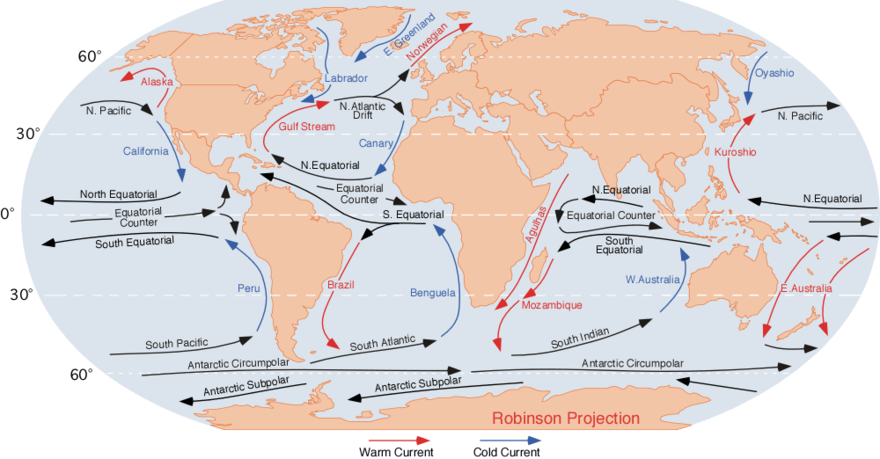
\includegraphics[width=0.9\textwidth]{表層洋流.png}
\end{figure}\FB
表層海流主要受行星風系影響。風海流係風所吹動,並受到科氏力作用形成艾克曼螺旋與西方強化作用,例如信風形成的南、北太平洋暖流。而補償流補償海水離開之處,大部分的涼流和湧升流為補償流,例如加利福尼亞涼流、秘魯涼流、秘魯湧升流。傾斜流則平衡海面高度,例如赤道逆流。這些洋流共同形成了多個環流(Circulation/Gyre),這些環流又組成表層環流系統。表層環流可以分為:
\begin{itemize}
\item 以中低緯海區的副熱帶高壓區為中心的反氣旋型大洋環流,存在於北太平洋、南太平洋、北大西洋與南大西洋。
\item 以北半球中高緯海區的低壓區為中心的氣旋型大洋環流,存在於北太平洋與北大西洋。
\item 盛行西風形成的西風漂流因無大陸阻擋在南極周圍形成西向東的南極繞極環流/環南極流(Antarctic Circumpolar Current, ACC)。環南極區域多溫帶氣旋發展,且無法大陸阻隔,是全球海面風速與浪高最大之處。
\item 北印度洋形成的季風環流。
\end{itemize}
\subsubsection{黑潮(Kuroshio Current, KC)}
黑潮北太平洋環流的一部分,為暖流,為全球第二大洋流,只居於墨西哥灣暖流之後。流速約為100至200公分每秒,厚度約500至1,000公尺,寬度約200公里,高溫高鹽度,因海水中懸浮物少,光反射率低,色深,故得名。\\
黑潮主流自赤道沿著東亞島弧移動,通過呂宋島東側與臺灣島東側,在臺灣東北至琉球群島一帶因海底地勢隆起而抬升,形成漁場。接著沿日本東側北上,於北緯35度附近部分東轉,形成北太平洋洋流,部分與南下的親潮(Oyashio current)/千島寒流(Okhotsk current)會合,形成西北太平洋漁場,是世界五大漁場之一,而後亦東轉匯入北太平洋洋流。\\
黑潮支流:
\begin{itemize}
\item 臺灣暖流(Taiwan Warm Current, TWC):夏季時,因為西南季風,南海表層流/南海暖流(South China Sea Warm Current, SCSWC)自向東北流動,部分在巴士海峽匯入黑潮主流,部分與黑潮支流一同進入臺灣海峽向北,稱臺灣暖流,在約北緯31度,與長江入海逕流形成的中國沿岸流/浙江-福建沿岸流(Zhejiang-Fujian Coastal Current, ZFCC)(涼流)相匯,形成流系分隔,並形成東海舟山漁場,接著在東海匯入黑潮主流,臺灣海峽東半側水溫在25°C以上。冬季時,因為東北季風,中國沿岸流較夏季強,南海表層流較夏季弱,臺灣海峽海流大致向南,烏魚沿中國沿岸流海流約20至22°C的海水南下產卵,為冬季臺灣海峽一帶之漁獲,黑潮支流在澎湖、雲彰一帶與中國沿岸流相匯,部分西轉往南海,臺灣海峽及東海西側由中國沿岸流主導的區域海溫在25°C以下,其東邊黑潮主導的區域海溫則在25°C以上。
\item 黃海暖流(Yellow Sea Warm Current, YSWC):黑潮支流,大致沿東經124度北上,然後通過渤海海峽流入渤海,形成不凍港。
\item 對馬(Tsushima)暖流:黑潮支流,自東海通過對馬海峽進入日本海,與利曼(Liman)寒流相匯,在北海道與本州之間的津輕海峽形成向東的津輕(Tsugaru)暖流。
\end{itemize}
\ssc{溫鹽環流(Thermohaline circulation, THC)}
\begin{figure}[H]
    \centering
    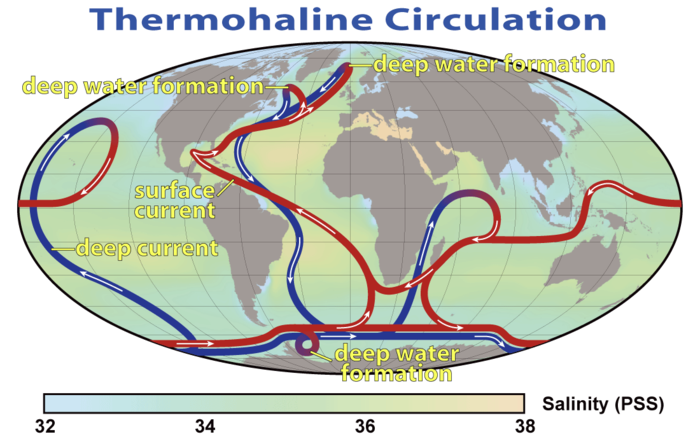
\includegraphics[width=0.9\textwidth]{THC.png}
\end{figure}\FB
由溫度和鹽度產生的海水密度梯度力所驅動的密度流,較表面風成流流速小許多,包含深層和底層洋流,帶動熱與鹽度的傳輸,平均週期一般認為是一千六百年。\\
極地冰層為淡水,融冰時形成的低鹽度冷水通常留在較淺處,結冰時排出鹽類形成的高鹽度冷水則下沉,形成NADW和AABW,是溫鹽環流的主要推動者。\\
深層海水為深海帶來富含氧氣的冷水,使深海好氧生物生存,在傳輸中因為其中生物的呼吸作用,使氧氣濃度下降、二氧化碳濃度提高,並因為其中生物的分解作用使養分增加,是湧升流會造成漁場的重要原因。
\sssc{北大西洋深層水(NADW, North Atlantic Deep Water)}
北極結冰的高鹽度冷水下沉,在北大西洋形成此水團,接著沿大西洋深層流向南方,並在南半球深層海洋中與其他深水流形成混合。
\sssc{南極底層水(AABW, Antarctic Bottom Water)}
南極洲周圍鹽度較北極高。南極結冰的高鹽度、低溫度、高密度水下沉,在南極洲附近形成此水團,接著流向大西洋、印度洋和太平洋的底部。
\sssc{北極中層水(AIW, Arctic Intermediate Water)}
來自北極地區水溫較低且鹽度較低的海流,在北大西洋中層海域流向南部,與NADW和其他水體混合。
\sssc{北太平洋深層水(NPDW, North Pacific Deep Water)}
與NADW類似,水溫較低、鹽度較高,於北太平洋流向南部,並在太平洋深層與其他深水流動混合。
\sssc{大西洋經向翻轉環流(AMOC, Atlantic Meridional Overturning Circulation)}
是溫鹽環流的重要組成部分。北大西洋海域,表層溫暖的鹹水向北流動(北大西洋暖流)輸送熱到北方,到達高緯後冷卻的水下沉,回到深層海水向南流動,即 NADW。
\sssc{深層西部邊界流(DWBC, Deep Western Boundary Current)}
主要由 NADW 和 AABW 組成,沿著大西洋西部邊界從拉布拉多海向南流至赤道。
\sssc{上升流}
深層與底層的舊水團歷經海洋混合而密度降低,因而在一些地方產生上升流回到淺層,沿加利福尼亞涼流、北赤道暖流、西澳暖流、南赤道暖流、阿古拉斯暖流、本吉拉涼流、墨西哥灣流、北大西洋暖流等表層洋流又可以回到兩極。一般認為存在於北太平洋、南冰洋與印度洋的某些地方。
\end{document}